\documentclass{article}

\usepackage[serbian]{babel}

\usepackage[letterpaper,top=2cm,bottom=2cm,left=3cm,right=3cm,marginparwidth=1.75cm]{geometry}

\usepackage{amsmath}
\usepackage{graphicx}
\usepackage[colorlinks=true, allcolors=blue]{hyperref}
\newcommand{\HRule}{\rule{\linewidth}{0.5mm}}

\begin{document}
	\vspace*{5cm}
	\thispagestyle{empty}
	\centerline{\huge \textbf{MATEMATIČKI FAKULTET}}
	\vspace{2cm}
	
	\begin{center}
		
		{\Large Seminarski rad}\\
		{\Large	iz Tehničkog i naučnog pisanja}\\
		\Huge\HRule\\[0.4cm] %0.4cm
		{Robotika u 2022.}\\
		\HRule \\[20pt] %20pt
		\begin{minipage}{0.4\textwidth}
			\begin{flushleft} \large
				{\Large Luka Matić}\\
				{\Large Marko Cvijetinović}
			\end{flushleft}
		\end{minipage}
		~
		\begin{minipage}{0.4\textwidth}
			\begin{flushright} \large
				{\Large Đuro Cerović} \\
				{\Large Mihajlo Radojević}\\ 
			\end{flushright}
		\end{minipage}\\[5cm]
		\Large{Beograd, Novembar 2022.}
	\end{center}
	\pagebreak
 \begin{abstract}
     Ovaj tekst je napravljen da vam prikaže napredak robotike do danas.\\
      U samom uvodu postoje neke činjenice i zakoni koje verovatne niste znali a odnose se na robote i robotiku. Obratite pažnju na to koliko je zapravo sama robotika i veštačka inteligencija u robotici napredovala a da niste ni primetili. Pomoću naučnih istraživanja i stručnjaka koji su istaživali i pisali o robotici, mi smo to prikupili u ovom radu, kako bi vam ukratko pokazali neke interesantne stvari i činjenice. Nadam se da ćete da uživate u našem radu i naći nešto korisno što će vam poslužiti.
    
 \end{abstract}
	\tableofcontents
    \pagebreak
	\section{Uvod}
	
	Danas je razvoj nauke i tehnike toliko ubrzan, da se svet nalazi u jednoj od perioda koje često nazivamo fazama revolucionarnih promena. Razvoj nauke i novih tehnologija, po mišljenjima mnogih, utiče na kvalitativne promene kako u proizvodnji, tako i u društvu uopšte.
	
	Visoka automatizacija u industriji dovodi do toga da se čovek bavi samo nadgledanjem proizvodnje.\\
	Razvijene zemlje su uvidele značaj i perspektivu novih tehnologija i ulažu sve više sredstava u razvoj istih. Jedna od grana ove tehnološke revolucije jeste robotika. Robotika je kombinacija inženjeringa, nauke i tehnologije koja rezultira uredjajima koji se nazivaju roboti. \cite{robotics2022,robots2022}
	
	
	
	Da bi smo razumeli pojam i značaj robotike, prvo treba da se upoznamo sa pojmom \href{https://www.sciencefriday.com/segments/the-origin-of-the-word-robot/}{"robot"}.\cite{word robot}
	Obično kada se pomene reč robot pomislimo na čovekolike robote iz filmova, transformerse pa čak robote koji rade u fabrikama. Danas je robotika razvijena do te mere, da postoji mnogo različitih vrsta robota kako u nauci i industriji, tako i u svakodnevnom životu. Robot je mašina sa automatskim upravljanjem koja zamenjuje ljudski napor, iako uglavnom ne liči na čoveka po izgledu ili po načinu obavljanja poslova. Dakle, robotika je grana uključuje koncepciju, dizajn, proizvodnju i rad robota. \cite{robots in nowdays}
	
	\subsection{Tri zakona robotike}
	Tri zakona robotike (eng. "Three laws of robotics") je osmislio pisac naučne fantastike Isak Asimov (\emph{engl.} Isaac Asimov). Prvi put se pojavljuju u njegovoj kratkoj priči "Kolo-naokolo" (\emph{engl.}"Runaround") iz 1942. godine, i oni glase \cite{three laws of robotics}:
	\begin{enumerate}
	\item \textbf{Robot ne sme povrediti ljudsko biće niti, svojom neaktivnošću, dozvoliti da ljudsko biće bude povređeno}.
	
	\item \textbf{Robot mora poštovati naređenja ljudskih bića, osim ako se ta naređenja ne kose sa prvim zakonom.}
	
	\item \textbf{Robot mora da štiti sopstvenu egzistenciju, osim ako se to ne kosi sa prvim i drugim zakonom.}
	\end{enumerate}
	
	Asimov je kasnije dodao još jedan zakon, \textbf{poznati kao četvrti ili nulti zakon}, koji prethodi ostalima. On glasi:"\textbf{Robot ne sme nauditi čovečanstvu niti, svojom neaktivnošću, dozvoliti da se čovečanstvu naudi"}.\par
	Tri zakona, kao i nulti, prožimaju naučnu fantastiku i navode se u mnogim knjigama, filmovima i drugim medijima, a takođe su uticali i na razmišljanje o etici veštačke inteligencije. \cite{three laws of robotics}
	
	
	\section{Saradnički roboti}
	
	Usled restrikcija postavljenih zbog COVID-19 pandemije, dolazi do sve veće potražnje za robotima koji bi komplementirali rad zaposlenih. Toliko, da popularnost saradničkih robota dovodi do nestajanja strepnji kako će roboti preuzeti poslove ljudima. Realnost je da oni pomažu ljudima da rade lakše i bezbednije dok riboti preuzimaju mesta nepoželjna za ljude.
	
	Saradnički roboti su, za razliku od uobičajenih, dizajnirani da rade sa ljudima, a ne u izolaciji. Ovo omogućava kompanijama da kombinuju prednosti ljudi i robota, što povećava produktivnost. \cite{robotics2022}
	
	Saradnički roboti mogu da rade suvoparne, prljave i opasne poslove koje su nekad izvršavali ljudi. To može biti od nezamisljive važnosti u državamsa sa većinski fakultetski obrazovanim stanovništvom, jer oni ne žele da se bave takvim poslovim pa dolazi do manjka radne snage.
	
	Pokrivanjem radnih mesta na nižem nivou, saradnički roboti omogućavaju ljudima da okupiraju više funkcije u kompanijama. Ne samo da ovo ide u korist radnicima, već je i moguće doći do veće efikasnosti i preciznosti jer za razliku od ljudi, automatizovana tehnologija nije sklona pravljenju grešaka.
	
	Povrh svega toga, roboti mogu da rade bez prestanka što očigledno povećava prihode, a i olakšava izvršavanje poslova zadatih u kratkom vremenskom roku. \cite{cobots}
	
	Saradnički roboti se često koriste u fabrikama, pakuju, raspakuju ili razmeštaju robu, kao što se vidi na slici \ref{cobot} ili rade kao čistači. \cite{robots2022}
	
	\begin{figure}
		\centering
		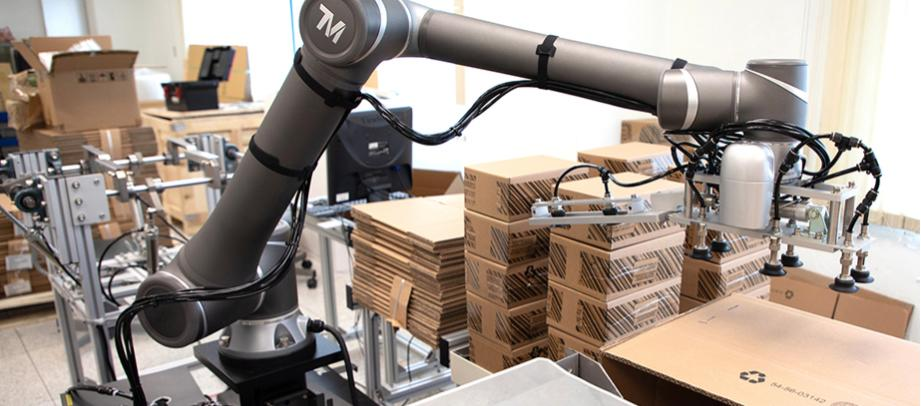
\includegraphics[scale=0.41]{Cobot.jpg}
		\caption{Slika preuzeta sa \url{https://kinemarobotica.com.}}
		\label{cobot}
	\end{figure}
	
	\section{Roboti dostavljači}
	Slično kao i saradnički roboti, ovaj trend je nastao usled COVID-19 epidemije zarad smanjenja kontakta između zaposlenih i mušterija jer to može dovesti do širenja zaraze.
	
	Automatizovana dostava hrane i ostalih manjih porudžbina je dostigla toliku popularnost za svega godinu ili dve, da neke Američke države već imaju zakone koje regulišu gde roboti dostavljači smeju da se kreću. Još jedna prednost robota u ovom poslu je fleksibilnost i u stanju su da obave i one porudžbine čija je isporuka zahtevana istog dana.
	\vspace{0.25cm}
	\begin{center}
		\begin{tabular}{ |p{1cm}|p{1cm}|p{1cm}|p{1cm} |p{1cm}|p{1cm}|p{1cm}|p{1cm}|p{1cm}|p{1cm}|p{1cm}|}
			\hline
			\multicolumn{11}{|c|}{Procenat isporuka koji je stigao u obećano vreme u SAD-u po mesecima} \\
			\hline
			Godina & Mart & April & Maj & Jun & Jul & Avgust & Sept. & Okt. & Nov. & Dec. \\
			\hline
			2019 & 88 & 89 & 89 & 89 & 89 & 89 & 87 & 88 & 86 & 75 \\
			2020 & 85 & 76 & 72 & 71 & 77 & 77 & 80 & 82 & 80 & 72 \\
			\hline
		\end{tabular}
	\end{center}
	\vspace{0.25cm}
	Zabeležava se rast broja porudžbina i smanjenje traženog roka isporuke iz godine u godinu, što doprinosi povećanju potražnje robota za dostavu. \cite{robotics2022, sameday}  
	
	\section{Prediktivno održavanje}
	Robotika može da uštedi ogromne količine novca tokom vremena, ali takođe dolazi sa troškovima održavanja kako bi se obezbedile vrhunske performanse. Kao rezultat, prediktivno održavanje je u porastu u robotici ove godine. Prediktivno održavanje koristi tehnologiju kao što su senzori Interneta stvari za praćenje performansi i fizičkog stanja robota. Podaci senzora otkrivaju pad performansi koji ukazuje kada je vreme da se završi održavanje pre nego što je potrebna velika popravka.
	
	IoT senzori su takođe korisni u robotskoj automatizaciji procesa, gde mogu da pomognu u vođenju robota u veoma korisnim zadacima, kao što je kontrola kvaliteta. IoT i tehnologije daljinskog otkrivanja i praćenja postaju posebno popularne u skladištima, gde se roboti koriste za sve, od sakupljanja artikala sa polica do pakovanja kutija za otpremu.
	\cite{robotics2022}
    \begin{figure}
     \centering
	   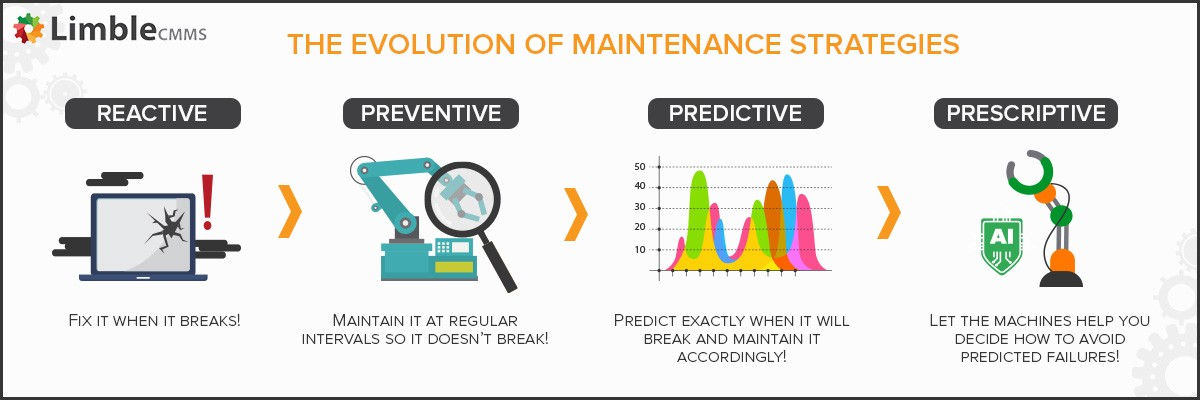
\includegraphics[scale=0.37]{dijagram.jpeg}
	   \caption{Prediktivno održavanje se odnosi na upotrebu proaktivnih metoda održavanja zasnovanih na podacima koje su dizajnirane da analiziraju stanje opreme i pomažu u predviđanju kada održavanje treba da se izvrši. (Slika preuzeta sa \url{https://www.heavy.ai/technical-glossary/predictive-maintenance}).}
    \end{figure}
   

\newpage
	\section{Povećanje kompatibilnosti}
	Sa toliko usvajanja i inovacija u robotici, raznovrsnost i prilagođavanje postaju briga za neka preduzeća. U 2022. sve više programera robotike ima to na umu. Industrijski stručnjaci su istakli trend ka saradnji \cite{4 Robotic Process Automation (RPA) trends to watch in 2022} u oblasti robotske automatizacije procesa ove godine, oslanjajući se na kombinovanje brojnih tehnologija za maksimalnu efikasnost.
	Ovaj trend obuhvata veštačku inteligenciju i mašinsko učenje, ali i druge robote. Proizvodnoj kompaniji, na primer, mogu biti potrebni potpuno različiti roboti za razne delove svog proizvodnog procesa ili za pravljenje brojnih proizvoda. Postaje tržišna prednost za robote da budu lako kompatibilni sa drugim, potpuno drugačijim robotima. Ovo je zanimljiv kontrast u odnosu na druge industrije, ali ukazuje na budućnost koja se oslanja na robote.
	\cite{robotics2022}
  

 
\section{Kuhinjski roboti}
Oblast robotike se jako brzo prosiruje u gotovo svakoj oblasti svakodnevnog zivota, kuhinjski roboti dobijaju posebnu pažnju. Iako je ljudima teško da povežu robotiku sa kuhinjskim poslovima. Iskreno malo je i čudno zamisliti robota kako pruzima ulogu nekog poznatog kuvara ili smišlja neki novi recept. Medjutim radnika tog profila je jako malo u prehrambenoj industriji, a preduzećima je potrebno rešenje koje može zadovoljiti potražnju za brzim uslugama oko hrane. Odličan primer robotike u ovoj industrijskoj oblasti je robot za pravljenje pice koji se u prodaji našao 2021.godine. Njegovo ime je "Robot za pravljenje pice" (\emph{eng}."Picnic pizza-making robot")\cite{robotics2022}. Model ovog robota u stanju je da napravi čak 100 porudžbina po satu, takodje je lak za rukovanje i nije potrebna neka prevelika obuka da bi se s njim rukovodilo. Ovaj izum bio je nagradjen od strane Nacionalnog udruženja restorana 2021. godine. Doprineo je tome da se reši manjak radnika u toj industrijskoj sferi ujedno je i povećao higijenske standarde restorana.\cite{foodservice robots}


\section{Primena veštačke inteligencije u robotici}
Kako se robotika razvijala uz nju se razvijala i vestacka inteligencija. Globalna studija Mek Kinsi (\emph{engl. }McKinsey)\cite{McKinsey} je 2021. godine
otkrila da je 56 \% biznisa koristilo veštačku inteligenciju bar za jednu funkciju koja im je donela brojne benefite. Na primer, kompanije su doživele od 1-2 \% skoka u prodaji dok su biznisi u industriji proizvodnje
imali i do 20 \% smanjenih troškova. Interesantno je da su te kompanije imale izveštaje za smanjene troškove nakon adopcije veštačke inteligencije
u periodu između 2019 i 2020 godine.\par
U 2022. godini veštačka inteligencija ostaje kao najprimenljiviji trend u robotici zato što njena primena nastavlja da se razvija. Biznisi mogu da integrišu veštačku inteligenciju u automatske sisteme robotike kako bi
kreirali pametnu automatizaciju. Procesi kao što su korisnička podrška i upravljanje zalihama mogu se  automatizovati što ne bi bilo moguće samo sa robotikom. Inovacije u mašinskom učenju, kompjuterskoj viziji i obradi prirodnog jezika samo će nastaviti da povećavaju popularnost veštačke inteligencije pored i unutar robotskih sistema.\cite{robotics2022} 


	\section{Zaključak}
 Život u 21. veku bio bi težak i praktično nemoguć bez korišćenja novih tehnoligija. Roboti kakve smo nekada mogli da vidmo samo u filmovima danas su realnost. Razvijene države se nakon COVID-19 sve više oslanjaju i ulažu u nove tehnologije, što znači da roboti polako zamenjuju ljude u teškim i monotonim poslovima. Ljudi će moći da zauzimaju više pozicije u kompanijama i da imaju više slobodnog vremena. Što se tiče svakodvnevnog života, roboti imaju široku primenu kao što su dostava hrane (roboti dostavljači), rad u kuhinji (kuhinjski roboti)...

 Robotika i veštačka inteligencija su usko povezani, što znači da se razvojem veštačke inteligencije koja je neophodna u robotici, unapredjuju i sami roboti i njihova efikasnost. 

 Nesumnjivo je da će razvojem robotike ljudima iz generacije u generaciju život i obavljanje poslova biti značajno olakšani, ali ipak trebati voditi računa prilikom korišćenja novih tehnologija, održavati iste i imati na umu da robot nikada ne sme prekršiti 4 zakona robotike.
	
\pagebreak

        
\pagebreak
\begin{thebibliography}{99}
	
	\bibitem{robotics2022}
	https://aijourn.com/the-7-most-innovative-trends-in-robotics-in-2022/
    AI Žurnal (\emph{engl.} The AI Journal) je vebsajt Toma Alena (\emph{engl.} Tom Allen) koji intervjuiše eksperte iz robotike.
	
	\bibitem{cobots}
	https://www.robotics247.com/article/collaborative\_robots\_raise\_the\_bar\_for\_productivity je vebsajt koji je napravljen u saradnji sa nekim kompanijama iz oblasti robotike i veštačke inteligencije.
	
	\bibitem{sameday}
	https://www.digitalcommerce360.com/ je vebsajt kompanije koja prati prodaju i performanse kompanija za digitalnu kupovinu.
	
	\bibitem{robots2022}
	https://www.marktechpost.com/2022/07/18/top-emerging-robotics-trends-in-2022/ Prathamesh Ingle je konsultantski pisac sadržaja u MarktechPost. Po zanimanju je mašinski inženjer i radi kao analitičar podataka. Marktechpost je kalifornijska platforma koja sadrži podatke o mašinskom učenju, dubokom učenju i istraživanju podataka.
 
	\bibitem{robots in nowdays}
	https://www.techtarget.com/whatis/definition/robotics  je američka kompanija i globalni lider u marketinškim i prodajnim uslugama. TechTarget ima kancelarije u Bostonu, Londonu, Minhenu, Njujorku, Parizu, San Francisku, Singapuru i Sidneju.
 
       \bibitem{three laws of robotics}
	https://www.britannica.com/topic/Three-Laws-of-Robotics Osnova Britanike Online je enciklopedija Britanika, najveća i najautoritativnija enciklopedija na svetu. Pored aktualnih članaka, ona uključuje mape, fotografije, ilustracije, video snimke, multimedijske isečke i godišnjake od 1993. godine.

        \bibitem{word robot}
     https://www.sciencefriday.com/segments/the-origin-of-the-word-robot/ je pouzdan\\ izvor informacija za vesti i zabavne naučne priče.
 
        \bibitem{4 Robotic Process Automation (RPA) trends to watch in 2022}
     https://enterprisersproject.com/article/2022/1/4-robotic-process-automation-rpa-trends-watch-2022 4 trenda robotske automatizacije procesa (RPA) koje treba pratiti u 2022 je zajednica koja pomaže CIO-ima (Glavni Službenik za informisanje) i IT liderima da reše probleme. Ovaj sajt vodi Kevin Casey koji pise o tehnologiji i poslovanju za razne publikacije.

      \bibitem{foodservice robots}
        https://www.therobotreport.com/picnic-pizza-making-robot-is-now-available/ je sajt koji donosi pouzdane izveštaje iz svih oblasti robotike.

         \bibitem{McKinsey}
        https://www.mckinsey.com/ McKinsey je globalna konsultantska firma za menadžment. Rade sa vodećim kompanijama u prvitanom, javnom i društvenom sektoru.
 
	
	
	
	
\end{thebibliography}

\pagebreak

\end{document}